\documentclass[tikz,border=8pt]{standalone}
\usepackage{tikz}
\usepackage{amsmath, amssymb}

\begin{document}

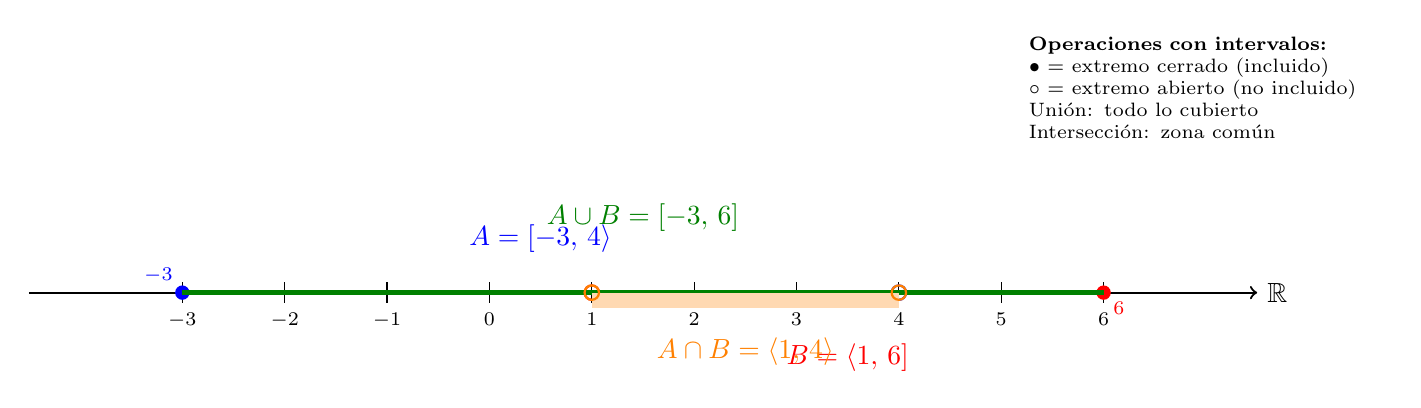
\begin{tikzpicture}[scale=1.3]

  % Recta real orientada
  \draw[->, thick] (-4.5,0) -- (7.5,0) node[right] {$\mathbb{R}$};
  \foreach \x in {-3,-2,-1,0,1,2,3,4,5,6}
    \draw (\x,0.1) -- (\x,-0.1) node[below] {\scriptsize $\x$};

  % Intervalo A = [-3, 4⟩
  \fill[blue] (-3,0) circle (2pt) node[above left] {\scriptsize $-3$};
  \draw[blue, thick] (-3,0) -- (4,0);
  \draw[blue, thick] (4,0) circle (2pt);
  \node[blue, above] at (0.5,0.3) {$A = [-3,\,4\rangle$};

  % Intervalo B = ⟨1, 6]
  \draw[red, thick] (1,0) circle (2pt);
  \fill[red] (6,0) circle (2pt) node[below right] {\scriptsize $6$};
  \draw[red, thick] (1,0) -- (6,0);
  \node[red, below] at (3.5,-0.4) {$B = \langle 1,\,6]$};

  % Unión A ∪ B = [-3, 6]
  \draw[green!50!black, ultra thick] (-3,0) -- (6,0);
  \node[green!50!black, above] at (1.5,0.5) {$A \cup B = [-3,\,6]$};

  % Intersección A ∩ B = ⟨1, 4⟩
  \fill[orange!30] (1,0) -- (4,0) -- (4,-0.15) -- (1,-0.15) -- cycle;
  \draw[orange, thick] (1,0) circle (2pt);
  \draw[orange, thick] (4,0) circle (2pt);
  \node[orange, below] at (2.5,-0.35) {$A \cap B = \langle 1,\,4\rangle$};

  % Leyenda
  \node[align=left, text width=4.5cm, font=\scriptsize] at (7, 2) {
    \textbf{Operaciones con intervalos:}\\
    $\bullet$ = extremo cerrado (incluido)\\
    $\circ$ = extremo abierto (no incluido)\\
    Unión: todo lo cubierto\\
    Intersección: zona común
  };

\end{tikzpicture}

\end{document}
